\documentclass[a4paper]{report}
\usepackage[french]{babel}
\usepackage[utf8]{inputenc}
\usepackage{graphicx} %'affichage des images
\usepackage[backend=bibtex]{biblatex}
\usepackage[T1]{fontenc}
\usepackage{listings}
\usepackage{xcolor}
\usepackage{wrapfig}

\definecolor{blue}{RGB}{38, 115, 255}
\definecolor{yellow}{RGB}{166, 122, 0}
\definecolor{red}{RGB}{166, 0, 0}

\lstdefinestyle{style1}{ 
    commentstyle=\color{yellow},
    keywordstyle=\color{blue},
    stringstyle=\color{red},
    basicstyle=\ttfamily\footnotesize,
    breakatwhitespace=false,
    breaklines=true,
    keepspaces=true,
    frame=L,
    language=python,
    keepspaces=true,
    showtabs=false,
}

\lstset{escapechar=@,style=style1}

\title{Rapport projet conception logicielle}
\author{Romuald GAFFE\and Yanis COSNEFROY\and Nguyen Phuong Vy VU\and Alexandre BOURGOIN}

\date{\today}

\begin{document}

\begin{titlepage}
    \centering
    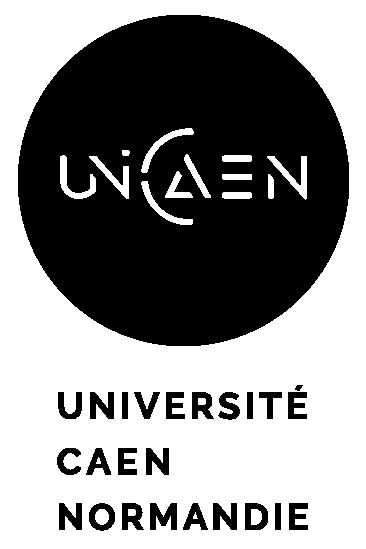
\includegraphics{images/logounicaen.png}\par\vspace{1cm}
    {\scshape\LARGE Rapport projet conception logicielle \par}
    \vspace{1cm}
    {\scshape\Large PyPuzzle\par}
    \vspace{1cm}
	{\Large Romuald GAFFE\par}
	{\Large Yanis COSNEFROY\par}
	{\Large Nguyen Phuong Vy VU\par}
	{\Large Alexandre BOURGOIN\par}
    \vspace{1cm}
	{\large \today \par}
\end{titlepage}

\tableofcontents
\part{Objectifs du projet}
\section{Présentation du concept}
Tout d'abord, nous avons choisi de créer un puzzle block puisque nous avions plus d'affinité et d'idées en rapport avec ce sujet. Nous voulions que ce jeu soit simple d'utilisation afin que tout le monde puisse y jouer. Le jeu que nous avons développé est composé de 4 modes de jeux, le premier étant le mode de jeu solo, il se présente sous forme d'une grille carré de 10 cases de côté. Le joueur obtient 3 pièces à placer sur la grille tirées aléatoirement parmi un total de 30 pièces(toutes orientations inclus). Les pièces qui apparaissent doivent toutes être placés dans la grille avant que les suivantes soit tirés. Si le tirage courant du joueur ne peut pas être placé alors un écran de fin de jeu s'affiche, montrant le score de la personne. Sur ce menu, le joueur aura la possibilité de retourner au menu principal ou de recommencer une partie. Ensuite le jeu se compose d'un mode multijoueur. Le premier étant contre une intelligence artificielle ayant le même mode de fonctionnement que le mode solo. Seul le score actuel de l'intelligence artificielle figure sur l'écran du joueur afin d'éviter d'en copier la stratégie. Le second mode multijoueur est, lui, un mode joueur contre joueur en local sur une même machine. Les grilles des joueurs s'affichent l'une après l'autre afin de limiter, de même, l'imitation de la stratégie adverse. Le dernier mode de jeu est un mode joueur contre joueur également mais en ligne où le but est de faire le plus de points.

\section{Cahier des charges}

\section{Exemples du jeux publiés}
Voici plusieurs block-puzzle provenant de jeux.fr, et des applications pour android: \\
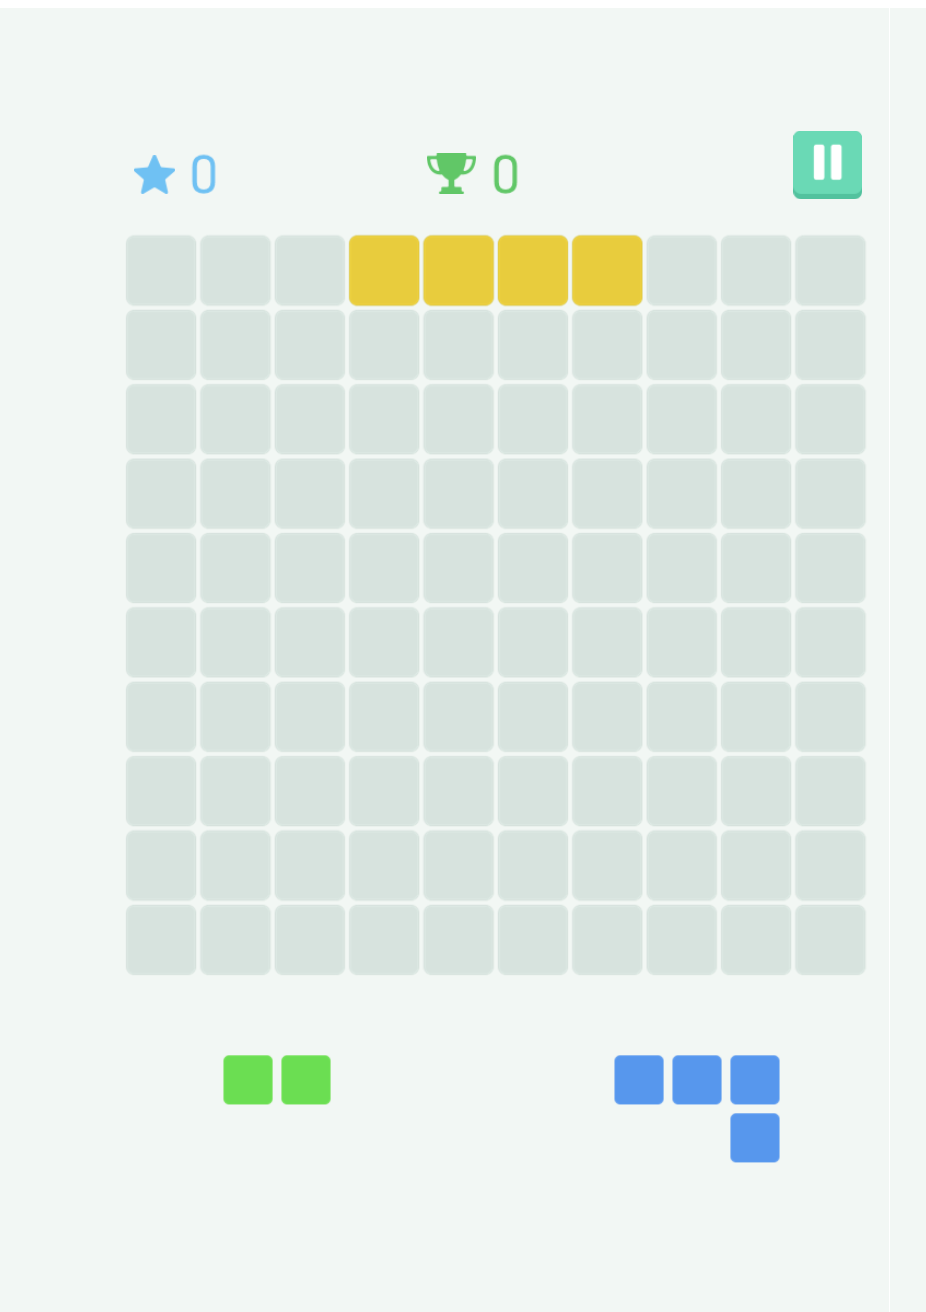
\includegraphics[height=180px]{images/jeuxPublie1.png}
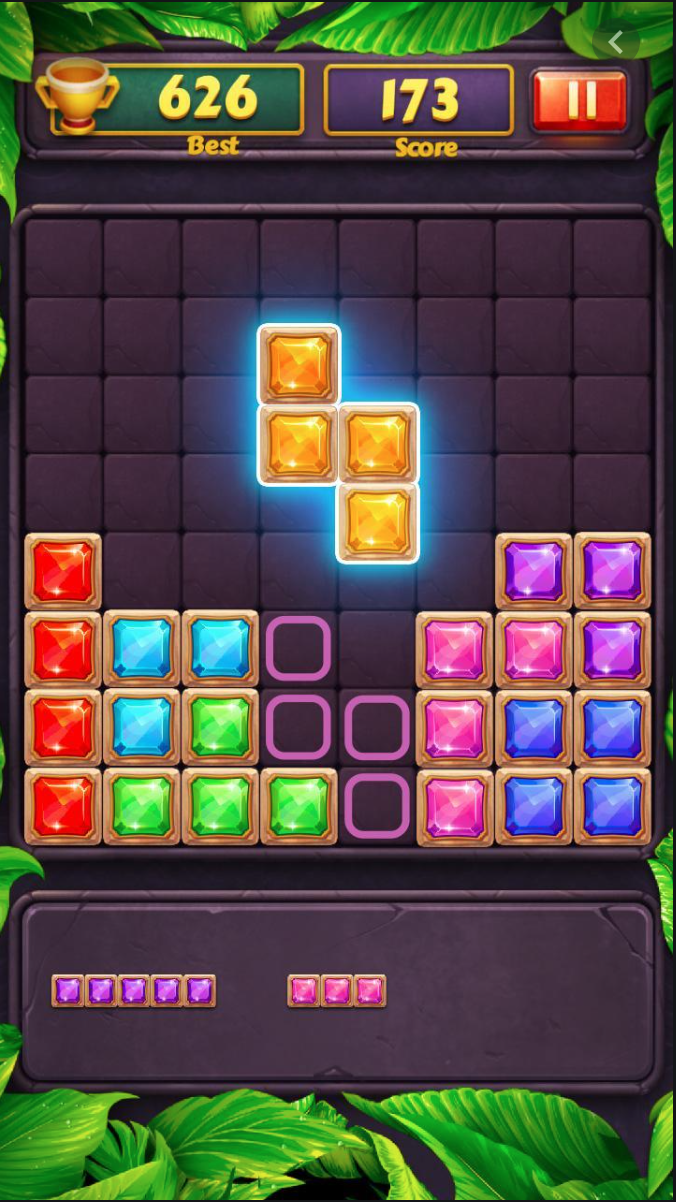
\includegraphics[height=180px]{images/jeuxPublie2.png}
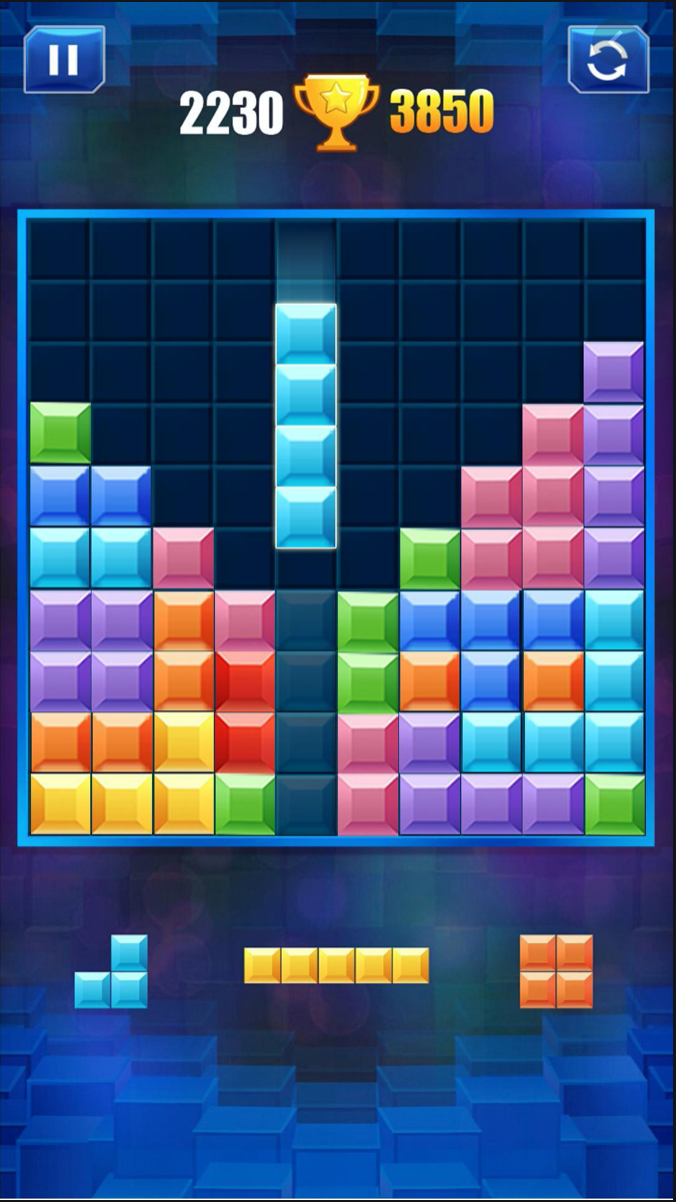
\includegraphics[height=180px]{images/jeuxPublie3.png}\\

On peut y retrouver les mêmes caractéristiques que notre projet. Notre projet a été conçu sur une base classique de block-puzzle qui réunit ces trois images montrées précédemment. Les différences entres ces block-puzzles et le nôtre sont l'aspect graphique ainsi que la sauvegarde du meilleur score établis sur le jeu par le joueur. On peut constater à l'essai de notre block-puzzle uniquement l'apparition des scores qui vont être actifs en fonction du jeu du joueur. Cependant nos règles sont un peu différentes par rapport au jeu déjà publié. On a décidé de ne pas rajouter de bonus ou d'aide à chaque fois qu'une ligne ou une colonne est remplie. C'est un choix volontaire pour provoquer une augmentation de concurrence de jeu avec d'autres joueurs mais aussi pour une adaptation plus développée de la difficulté de jeu. 
\part{Fonctionnalités implémentés}
\section{Mode solo}
\begin{wrapfigure}{R}{0.35\textwidth}
    \centering
    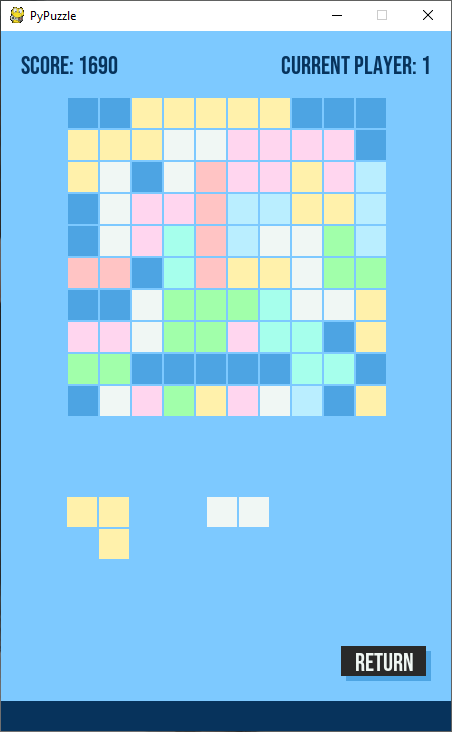
\includegraphics[width=0.3\textwidth, trim=0pt 0pt 0pt 30pt]{images/3-ingame.png}
    \caption{Gameplay solo}
\end{wrapfigure}
Tout d'abord la structure du jeu en mode solo est une structure de jeu plutôt classique comme on peut le voir dans l'image présente ci-dessous :\\

Comme on peut le constater à l'image du projet, il y a une grille placée au centre de la fenêtre qui possède une taille fixe. Autour de cette grille, va se trouver des informations essentielles pour le joueur comme son score actuel qui est placé en haut à gauche de la fenêtre. À droite, va se trouver le joueur qui joueur qui joue au jeu. En dessous de la grille, on va retrouver les 3 blocs de départ que le joueur devra placer dans la grille. Enfin, tout en bas à droite, il va y avoir un bouton pour permettre à l'utilisateur de retourner au menu du jeu. \\

Ensuite, les règles du jeu vont s'appliquer au fur et à mesure du jeu du joueur. Quand un block sera placé dans la grille, il va y avoir un ajout de 30 points à son score. Et dès qu'une ligne ou une colonne sera remplie, il va y avoir une disparition de la ligne ou de la colonne voir même les deux si les conditions sont réunies. Le bonus de point sera alors de 100 points lorsqu'une ligne ou une colonne est construite par l'utilisateur. Le joueur ne peut pas mettre sa partie en pause. Cependant, il n'y a pas de limite de temps. Dès que les trois blocs sont placés dans la grille, trois autres bloques vont réapparaître avec une probabilité de difficultés qui est calculée en fonction du score. \\

\begin{wrapfigure}{L}{0.35\textwidth}
    \centering
    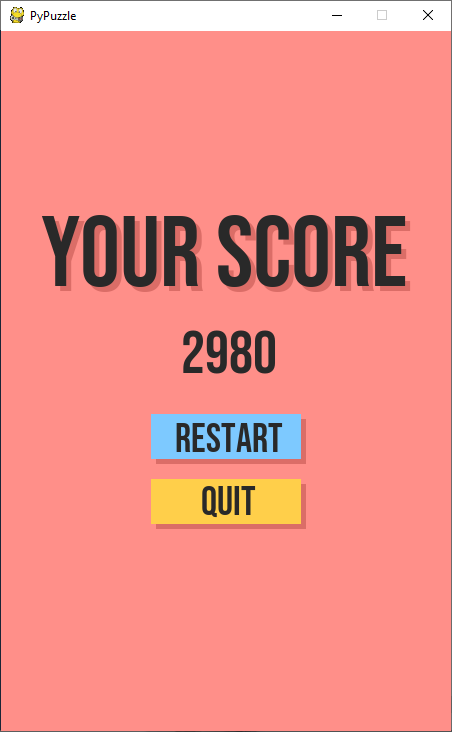
\includegraphics[width=0.3\textwidth, trim=0pt 0pt 0pt 50pt]{images/4-end.png}
    \caption{Gameplay solo}
    \vspace{-20pt}
\end{wrapfigure}

Enfin, si je le joueur perd en étant bloqué sur le placement impossible d'une pièce dans la grille, alors le jeu s'arrêtera et affichera un Game Over montré ci dessous avec les information de jeu du joueur : \\

Comme on peut le voir sur cette photo, le score du joueur est affiché. Afin d'éviter au joueur de repartir dans le menu pour relancer une partie, il a la possibilité de la relancer directement grâce au bouton "restart". Il a aussi la possibilité de quitter le jeu en cliquant sur le bouton "quit". Si le joueur veut retourner au menu, alors il devra d'abord recommencer une partie et cliquer sur le bouton "return" se trouvant en bas à droite de la fenêtre. 

\pagebreak

\section{Mode multijoueur}
\begin{wrapfigure}{R}{0.35\textwidth}
    \centering
    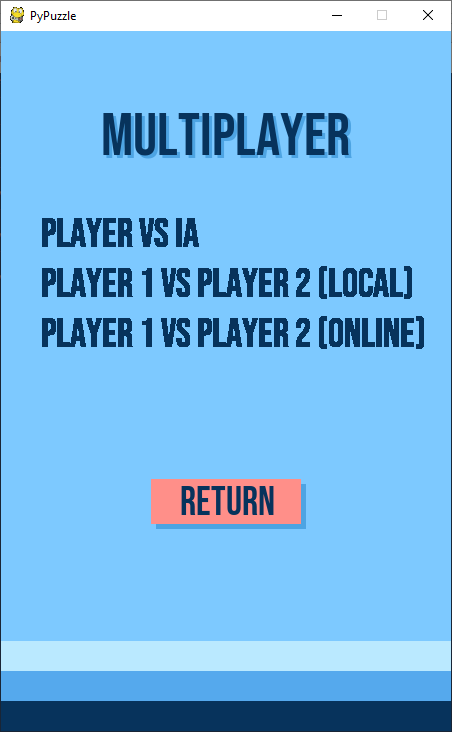
\includegraphics[width=0.3\textwidth, trim=0pt 0pt 0pt 150pt]{images/2-menumulti.png}
    \caption{Menu multijoueur}
    \vspace{-20pt}
\end{wrapfigure}
Différents modes de multijoueur sont présents dans ce projet. On peut y retrouver un multijoueur où un joueur réel va jouer contre une intelligence artificielle, un multoujoueur ou deux joueur vont s'affronter. Et enfin un multijoueur en réseau où deux joueur vont pouvoir s'affronter sur deux écrans séparés. En dessous va se trouver une photo ou va être représenté le menu du multijoueur. On va aussi y retrouver la possibilité d'un retour au menu principal dans le menu du multijoueur si le joueur veut jouer seul.\\


\subsection{Joueur vs Intelligence artificielle}
\begin{wrapfigure}{L}{0.35\textwidth}
    \centering
    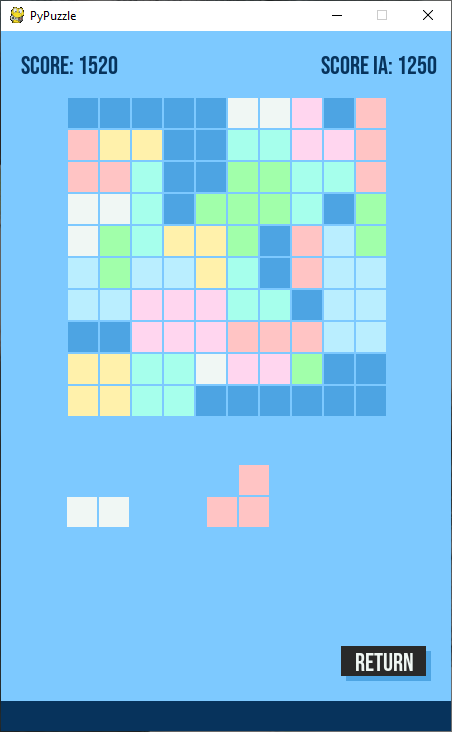
\includegraphics[width=0.3\textwidth, trim=0pt 0pt 0pt 30pt]{images/3-playwithai.png}
    \caption{Joueur vs IA}
    \vspace{-10pt}
\end{wrapfigure}
Tout d'abord, il faut savoir que le mode multijoueur avec le joueur contre l'intelligence artificielle se joue comme le mode solo. Le joueur va pouvoir jouer comme il voudra. Il n'aura pas accès à la grille de l'intelligence artificielle pour éviter de la tricherie. Cependant le joueur pourra jouer une fois sur deux. Le premier tour est commencé par l'intelligence artificielle puis est suivie du joueur se trouvant derrière l'écran. L'utilisateur va avoir comme information sa grille, ses points, les points de son adversaire, donc ici de l'intelligence artificielle et de ses blocs. Le joueur et l'intelligence artificielle vont tout les deux avoir les mêmes blocs pour que les difficultés soient égales de chaque côté. Le joueur va pouvoir retourner au menu si il le souhaite, toujours grâce au bouton se trouvant en bas à droite. Ci dessous, va se présenter une photo de la grille du jeu avec les différentes informations énoncées précédemment que le joueur va avoir.\\

\begin{wrapfigure}{R}{0.35\textwidth}
    \centering
    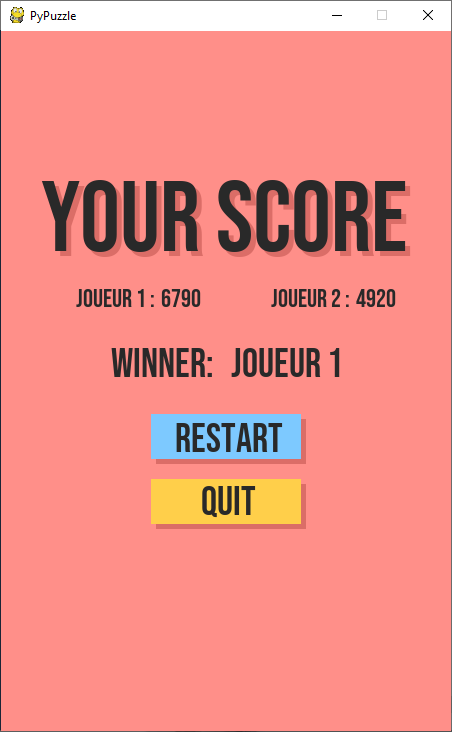
\includegraphics[width=0.3\textwidth, trim=0pt 0pt 0pt 30pt]{images/4-endmulti.png}
    \caption{Fin du jeu multi}
\end{wrapfigure}
Ensuite les règles du jeu sont les mêmes que pour le solo. Il n'y a pas de mise difficultés pour qui que ce soit car si l'un rempli une ligne ou une colonne, l'autre ne va pas recevoir de pièce qui peut le mettre en difficulté. Ici il y a juste une concurrence au niveau des points qui va justement permettre de départager la victoire entre le joueur et l'intelligence artificielle.\\

Enfin, si je le joueur perd en étant bloqué sur le placement impossible d'une pièce dans la grille, alors le jeu s'arrêtera et affichera un Game Over montré ci dessous avec les information de jeu du joueur. Si le jeu ne s'arrête pas c'est qu'il y a encore une possibilité de jouer.  \\

Comme on peut le voir sur cette photo, le score du joueur ainsi que celui de l'intelligence artificielle sont affiché. De plus on a décidé de rajouter une ligne pour faire ressortir le gagnant de la partie. Dans cette image, Player1 est le joueur se trouvant derrière l'écran et Player2 est l'intelligence artificielle. Afin d'éviter au joueur de repartir dans le menu pour relancer une partie, il a la possibilité de la relancer directement grâce au bouton "restart". Il a aussi la possibilité de quitter le jeu en cliquant sur le bouton "quit". Si le joueur veut retourner au menu, alors il devra d'abord recommencer une partie et cliquer sur le bouton "return" se trouvant en bas à droite de la fenêtre. 

\subsection{Joueur vs Joueur en local}
\subsection{Joueur vs Joueur en ligne}

\part{Éléments techniques}
\section{La grille}
La grille est mise sous la forme d'une classe, 
\section{Les pièces}
\section{L'aléatoire}
\section{L'intelligence artificielle}
\section{Le réseau}
\section{L'interface graphique}
Pour l'interface du jeu, on utilise \textbf{\textit{Pygame}}, une bibliothèque graphique dédiée aux jeux vidéos. 
Pygame n'est pas fourni avec Python. Donc, pour jouer, vous devrez télécharger et installer Pygame à la place. Pour appliquer Pygame:
\begin{lstlisting}
    import pygame @\color{blue}as@ pg
\end{lstlisting}

On va utiliser pygame pour faire et design l'interface du jeu, pas utiliser les images déjà faits et les mettre dans le jeu.
Et on va appliquer en même méthode pour faire le menu démarrer, le menu multijoueur et le menu de la fin du jeu.

\subsection{Le menu}
D'abord, il faut faire un réglage des tailles des positions. \textbf{\textit{pygame.Rect()}} n'est pas dessiner un rectangle, juste déterminé les tailles et les positions d'un rectangle.
\begin{lstlisting}
    #tailles de fenetre
    SCREENHEIGHT = 700
    SCREENWIDTH = 450
    screensize = (SCREENWIDTH, SCREENHEIGHT)
    #positions de la grille
    boardX = 65
    boardY = 65
    #tailles et positions des boutons
    soloButtonRect = pg.@\color{blue}Rect@(150, 318, 150, 50)
    multiButtonRect = pg.@\color{blue}Rect@(150, 383, 150, 50)
    quitButtonRect = pg.@\color{blue}Rect@(150, 448, 150, 45)
\end{lstlisting}

Pour commencer le jeu, on doit appeler la fonction \textbf{\textit{pygame.init()}}, elle doit être appelée en premier pour que de nombreuses fonctions Pygame fonctionnent
\begin{lstlisting}
    pg.@\color{blue}init()@
\end{lstlisting}

Ensuite, on doit construit un boucle pour tout le menu. Si une boucle est toujours vrai, alors elle fonctionne pour toujours.
\begin{lstlisting}
    def menu():
    doContinue = True
    while doContinue:
        for event in pg.event.get():
            if event.@type@ == pg.QUIT:
                fnc.quitGame() #dans function.py pour quitter
\end{lstlisting}

Puis, on ajoute des boutons, on utilise \textbf{\textit{.collidepoint()}} pour déterminer les positions des boutons.
\begin{lstlisting}
                elif event.@type@ == pg.MOUSEBUTTONDOWN:
                if soloButtonRect.@\color{blue}collidepoint@(@\color{blue}event.pos@):
                    solo() #autre menu pour basculer entre eux
                if multiButtonRect.@\color{blue}collidepoint@(@\color{blue}event.pos@):
                    multiMenu() #autre menu pour basculer entre eux
                if quitButtonRect.@\color{blue}collidepoint@(@\color{blue}event.pos@):
                    fnc.quitGame() #dans function.py pour quitter
        pg.display..@\color{blue}flip@() #pour mise a jour
\end{lstlisting}

Ensuite, on construit une interface d'affichage dans une autre fichier appelée \textbf{display.py}. 
Pour les textes, on utilise \textbf{\textit{pygame.font}} avec les sous-éléments \textbf{\textit{pygame.font.Font()}}, \textbf{\textit{"nom".render()}} et l'élement \textbf{\textit{"screen".blit()}}. 
Pour les rectangles (boutons), on utilise \textbf{\textit{pygame.draw.rect()}}.
Et pour colorer le fond, on utilise \textbf{\textit{"screen".fill()}}.

\begin{lstlisting}
    NAVY = (7, 51, 92)
    pg.font.@\color{blue}init()@
    bigFont = pg.font.@\color{blue}Font@('assets/BebasNeue-Regular.ttf', 100)
    pypuzzle = bigFont.@\color{blue}render@("PyPuzzle", True, NAVY)

    def displayMenu(win):
    win.@\color{blue}fill@(BACKGROUNDCOLOR)
    pg.draw.@\color{blue}rect@(win, BOARDCOLOR, (155, 323, 150, 45))
    pg.draw.@\color{blue}rect@(win, BOARDCOLOR, (155, 388, 150, 45))
    pg.draw.@\color{blue}rect@(win, BOARDCOLOR, (155, 453, 150, 45))
    #titre
    win.@\color{blue}blit@(pypuzzleShadow, (82, 170))
    win.@\color{blue}blit@(pypuzzle, (78, 165))
    #decoration
    pg.draw.@\color{blue}rect@(win, LIGHTBLUE, (0, 610, 450, 30))
    pg.draw.@\color{blue}rect@(win, BLUE, (0, 640, 450, 30))
    pg.draw.@\color{blue}rec@t(win, NAVY, (0, 670, 450, 30))
\end{lstlisting}

Pour les son, on utilise \textbf{\textit{pygame.mixer}} avec les sous-éléments \textbf{\textit{pygame.mixer.Sound()}}, \textbf{\textit{"nom".play()}} et \textbf{\textit{"nom".stop()}}.
Type de fichier est .wav (Les formats de fichiers audio pris en charge par Pygame sont MID, WAV et MP3.)
\begin{lstlisting}
    pg.mixer.@\color{blue}init@() #pour fonctioner
    soundMenu = pg.mixer.@\color{blue}Sound@("assets/menu.wav")
    soundMenu.@\color{blue}play@(-1, 0, 0)
\end{lstlisting}

On juste utilise une animation, c'est le survol quand on entre les boutons.
Ici, on utilise \textbf{\textit{pygame.mouse}} avec le sous-élement \textbf{\textit{pygame.mouse.get\_pos()}}.
pour déterminer les positions de la souris.
\begin{lstlisting}
    # HOVER
    pos = pg.mouse.@\color{blue}get\_pos()@
    if 340 + 85 > pos[0] > 340 and 615 + 30 > pos[1] > 615:
        pg.draw.@\color{blue}rect@(screen, dsp.YELLOW, (340, 615, 85, 30))
        screen.@\color{blue}blit@(dsp.returnMenuText, (354, 617))
    else:
        pg.draw.@\color{blue}rect@(screen, dsp.GRAY, (340, 615, 85, 30))
        screen.@\color{blue}blit@(dsp.returnMenuText1, (354, 617))
\end{lstlisting}

\subsection{Gameplay}


\part{Architecture du projet}
\section{Diagrammes des modules et des classes}
\section{Cas d'utilisation}

\part{Expérimentations et usages}
\section{Capture écrans}
Les captures ci-dessous rendront le joueur passionné de jouer au jeu.
\begin{enumerate}
    \item Menu démarrer avec animation de survol.\\
        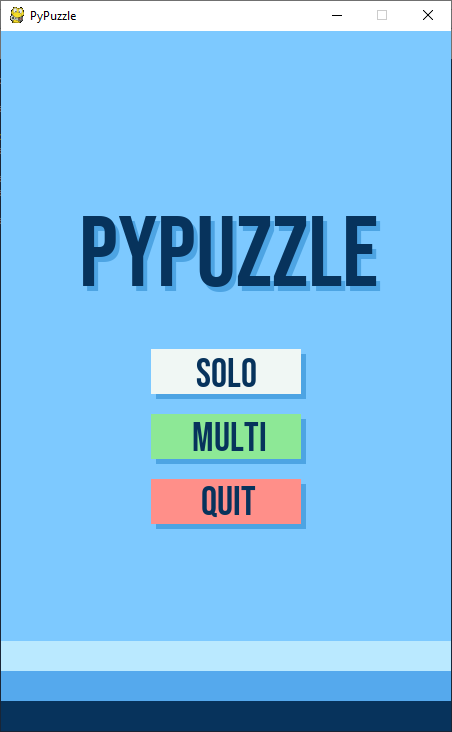
\includegraphics[scale=0.3]{images/1-menu.png}
        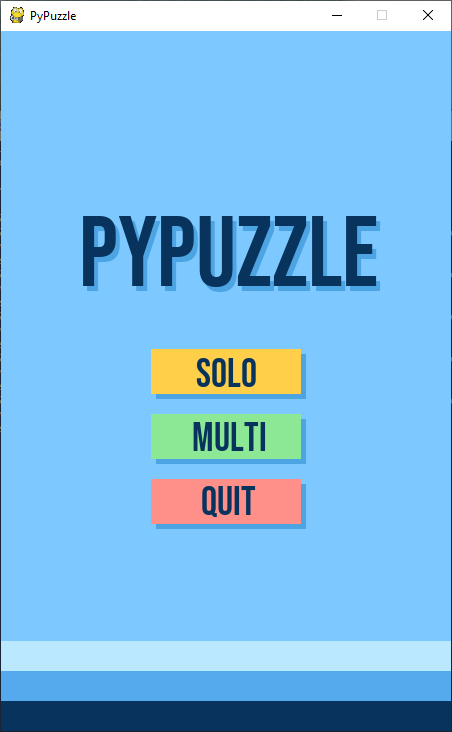
\includegraphics[scale=0.3]{images/1-ani.png}
    \item Menu multijoueur avec animation de survol.\\
        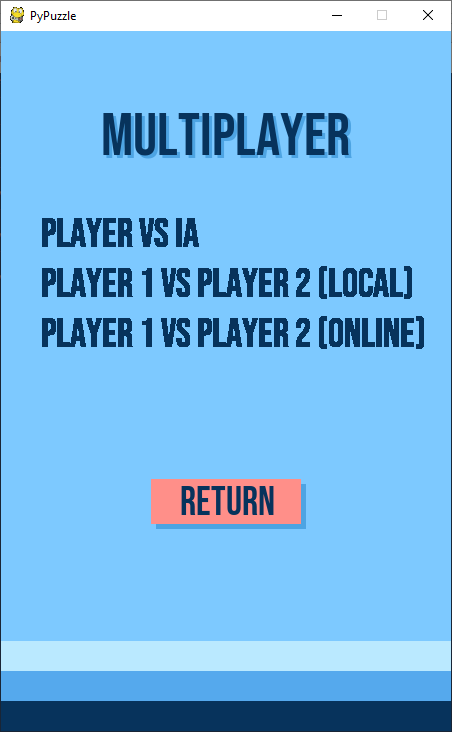
\includegraphics[scale=0.3]{images/2-menumulti.png}
        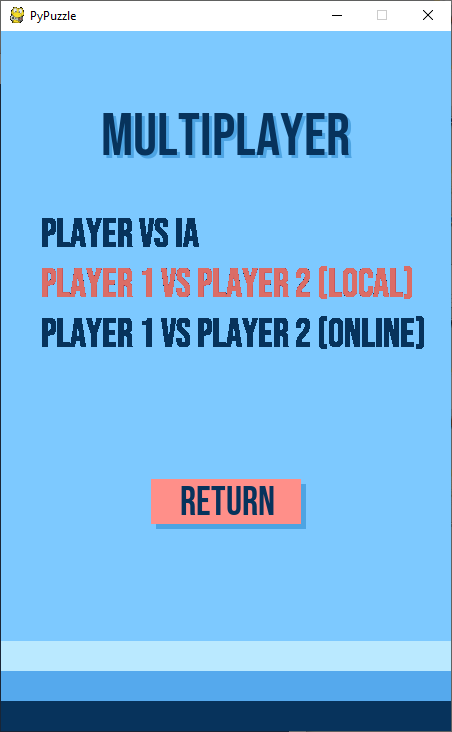
\includegraphics[scale=0.3]{images/2-ani.png}
    \item Gameplay (solo et multi). De nombreuses couleurs permettent au joueur de continuer et de ne pas s'ennuyer quand on joue.\\
        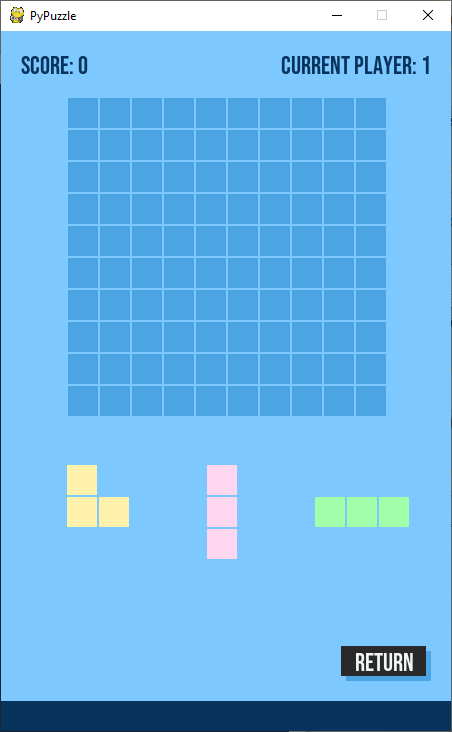
\includegraphics[scale=0.3]{images/3-ingamestart.png}
        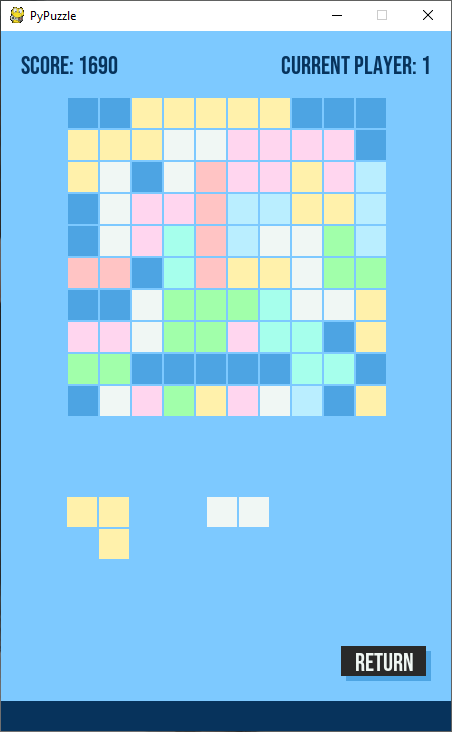
\includegraphics[scale=0.3]{images/3-ingame.png}
        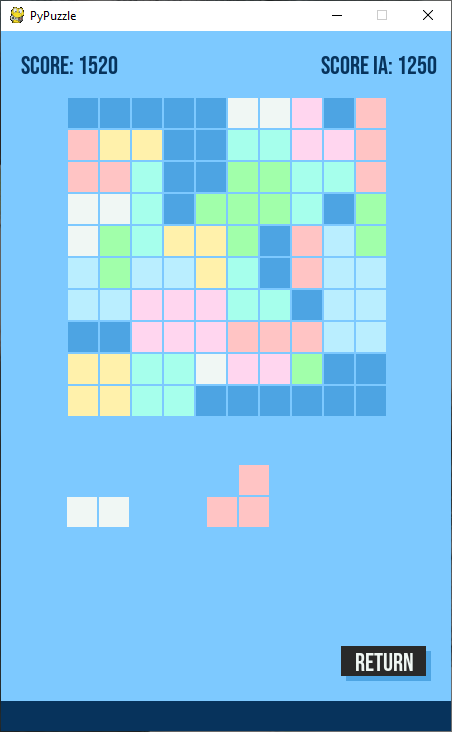
\includegraphics[scale=0.3]{images/3-playwithai.png}
    \item Fin du jeu avec animation de survol.\\
        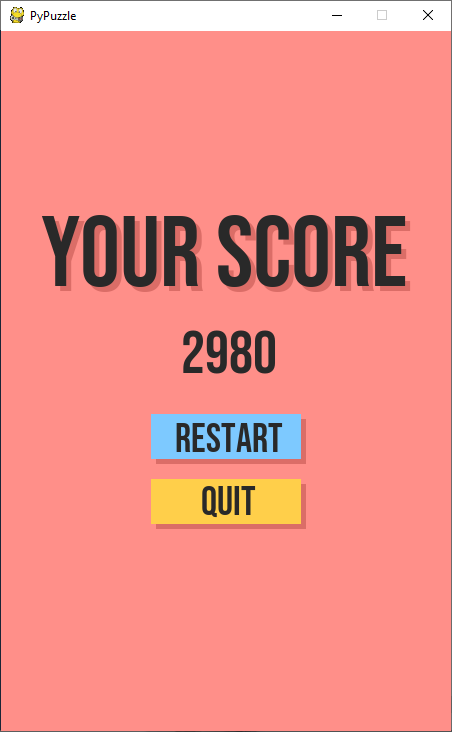
\includegraphics[scale=0.3]{images/4-end.png}
        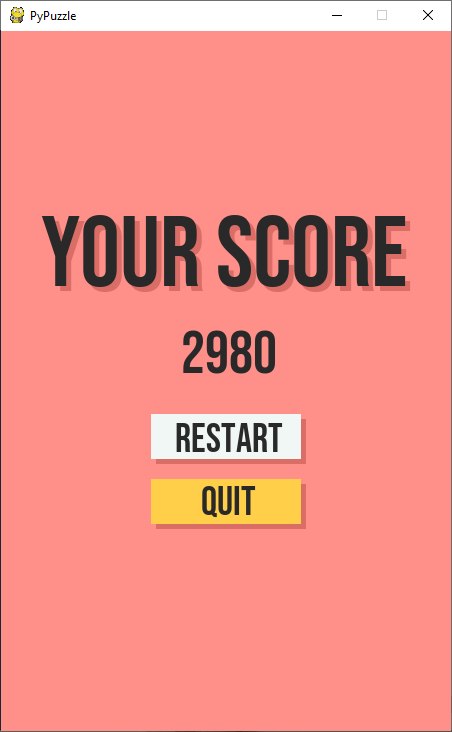
\includegraphics[scale=0.3]{images/4-endani.png}
        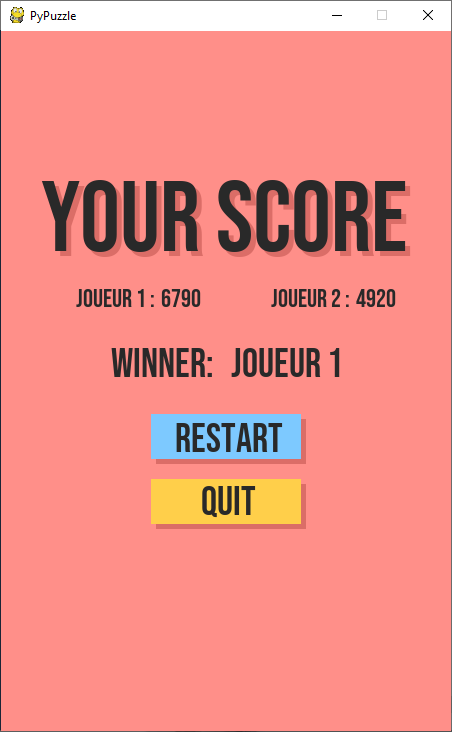
\includegraphics[scale=0.3]{images/4-endmulti.png}
\end{enumerate}


\section{Mesures de performance}

\subsection{Interfaces graphiques} 
Quelle est l'interface du jeu pour vous? Selon nous, après le contenu du jeu, l'interface du jeu est la plus importante pour attirer les joueurs.
C'est un jeu pour tout le monde, on choisit le minimalisme avec
une palette des couleurs pastels car ce sont les couleurs douces et pas sombre. 
Elle fait une atmosphère relaxée quand on le joue. Échouer mais pas en colère.\\

\begin{itemize} 
    \item Font: Bebas Neue Regular (Free Copyright)
    \item Couleur principale: \textbf{bleu(125, 201, 255)}
    \item Couleurs des pieces: les couleurs pastels\\
        
\includegraphics[scale=0.3]{images/palette1.png}
    \item Couleurs de menu\\
        
\includegraphics[scale=0.3]{images/palette2.png}
\end{itemize}

\subsection{Effet sonore}
On voulait ajouter de la musique à notre jeu, car on pensait que cela attirerait les joueurs. 
Comme la musique est quelque chose de très populaire à partir de maintenant, on pensait que les 
joueurs aimeraient que on ajoute de la musique au jeu que on a créé.\\

Au début du jeu, pas de bruit tonitruant, pas de son nervosité, on souhaite de mettre les conforts et les joyeux en joueant en premier. C'est pourquoi on choisit l'accord de base au piano C(Do) majeur.
Ensuite, le son des boutons est la note F(Fa) correspond à la première note de son du menu.
Puis, quand on joue, il n'y a pas de son au fond, il existe que le son des pièces pour que l'on se sent concentrer. Il faut savoir que l'on n'oublie pas que on est entraine de jouer au jeu donc le son du bongo apparait quand on glisse-despose les pièces.
Enfin, on choisit l'accord guitare C(Do) mineur, on pense à créer une synchronisation de la musique.


\part{Conclusion}


\end{document}
